\chapter{Introduction}

This chapter mainly provides a brief introduction to the entire project. Section \ref{bckgrd} gives the background of the project and some basic concepts. Section \ref{prodef} defines the problems of this project to be solved. Section \ref{fcswrk} gives a brief introduction to the proposed new model. Section \ref{thsorg} gives the structure of this thesis for the convenience of readers.

\section{Background}\label{bckgrd}

In this section, the background of this project is introduced. Subsection \ref{arlimg}, \ref{imgseg} and \ref{geosha} focus on aerial images, image segmentation and the segmentation with geometry respectively.

\subsection{Aerial Image}\label{arlimg}

An aerial image is a projected image which is ``floating in air'', and cannot be viewed normally. It can only be seen from one position in space, often focused by another lens (from Wikipedia). In this project, aerial images generally refer to satellite images, which are taken from satellites flying around the earth. These kind of images have an extremely wide range of applications in the field of geographical surveying and mapping. It can not only clearly depict the terrain but can also show the structure and the layout of the city. Furthermore, it can also provide services such as land use status and remote sensing monitoring.

Nowadays, many buildings are constantly being updated in real life and many landscapes are changing with natural activities. Therefore, electronic maps need to be updated accordingly, and aerial images can provide those maps with important references. Figure \ref{fig:egsatimg} shows two examples of aerial images.

\begin{figure}[!h]
	\centering
	\subbottom[an area of Zurich\label{fig:egzurich}]{
		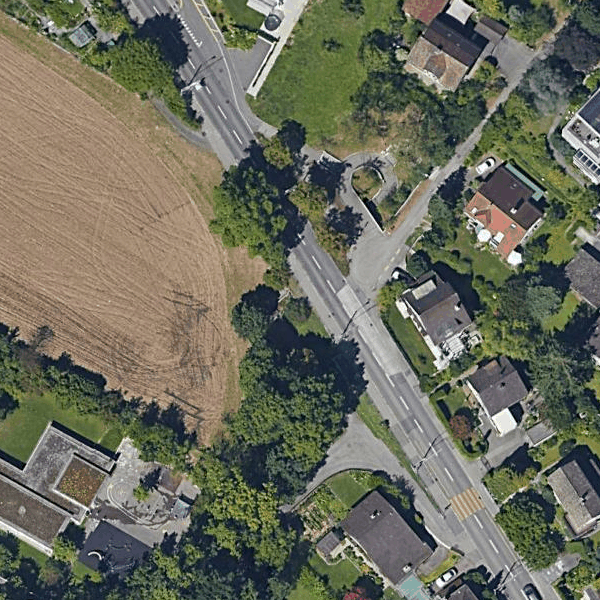
\includegraphics[width=\figfig\textwidth]{1-00-0.png}
	}
	\subbottom[an area of Chicago\label{fig:egchicago}]{
		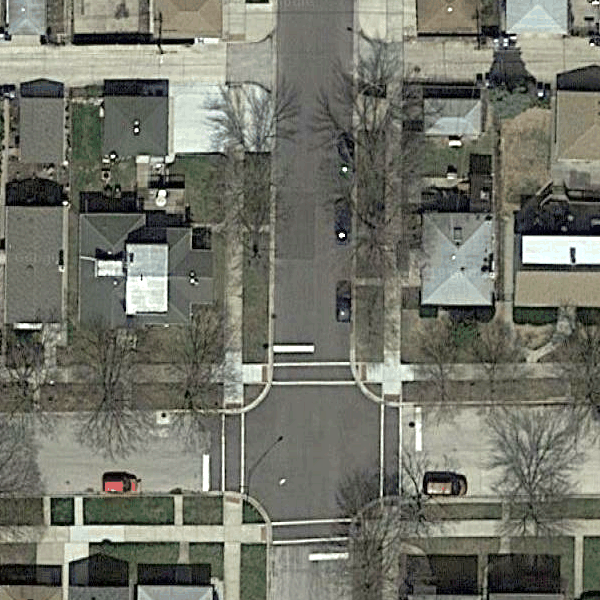
\includegraphics[width=\figfig\textwidth]{1-00-1.png}
	}
    \caption[Example of two satellite images]{Example of two satellite images.}
	\label{fig:egsatimg}
\end{figure}

\subsection{Image Segmentation}\label{imgseg}

In computer vision, image segmentation is the process of partitioning a digital image into multiple segments (sets of pixels, also known as super-pixels). The goal of segmentation is to simplify and change the representation of an image into something that is more meaningful and easier to analyze (from Wikipedia). In fact, image segmentation is a process of labelling each pixel in an image. Pixels with the same label are generally similar in the metric of certain visual characteristics, such as color, brightness or texture. Adjacent areas are usually very different under this metric.

Specifically, binary image segmentation is to label each pixel as 0 or 1. Figure \ref{fig:eg01imgseg} shows an example of binary image segmentation, where the original image is basically segmented as foreground and background.

传统的图像分割技术是为图像中的每一个像素打label。如用0表示,1表示,2表示。航拍图像的图像分割指的是在航拍图像中提取出房屋、道路。(给例子)然而这样的表示方式有很多的局限性——如无法对房屋进行定位、存储上对每个像素,很废空间什么的。

\begin{figure}[!h]
	\centering
	\subbottom[original image\label{fig:egbfrseg}]{
		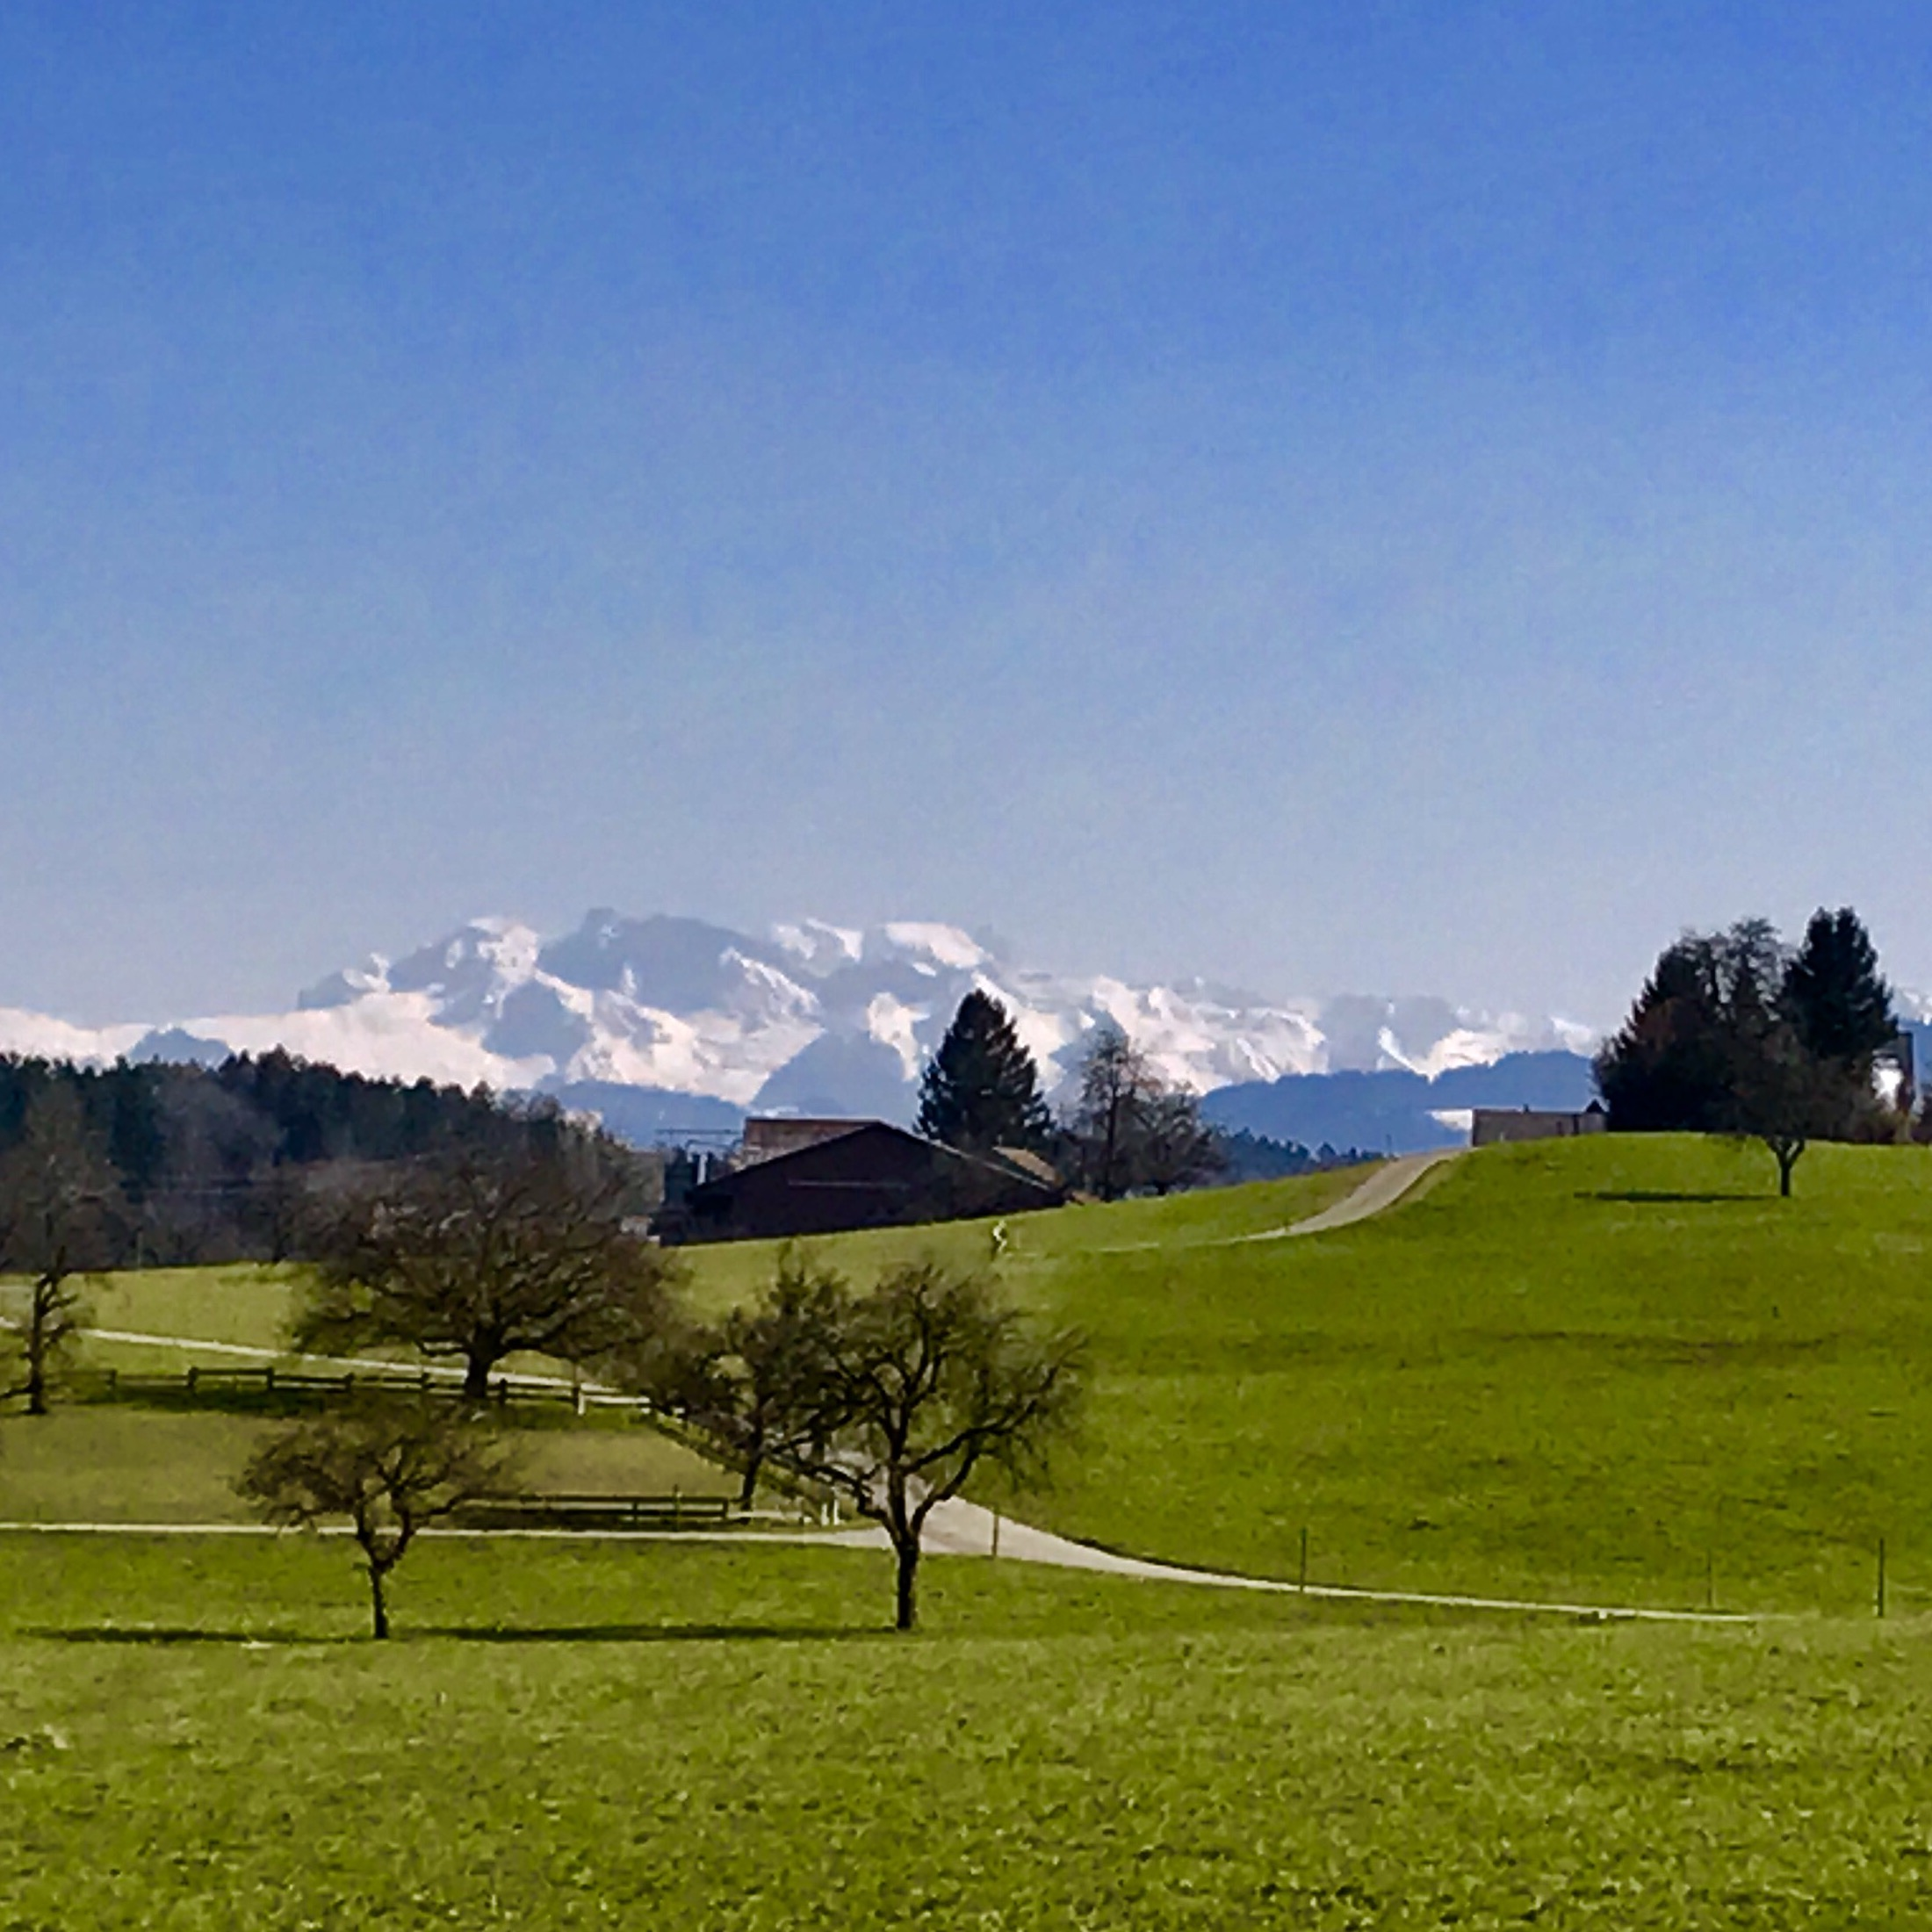
\includegraphics[width=\figfig\textwidth]{1-01-0.jpg}
	}
	\subbottom[image after segmentation\label{fig:egaftseg}]{
		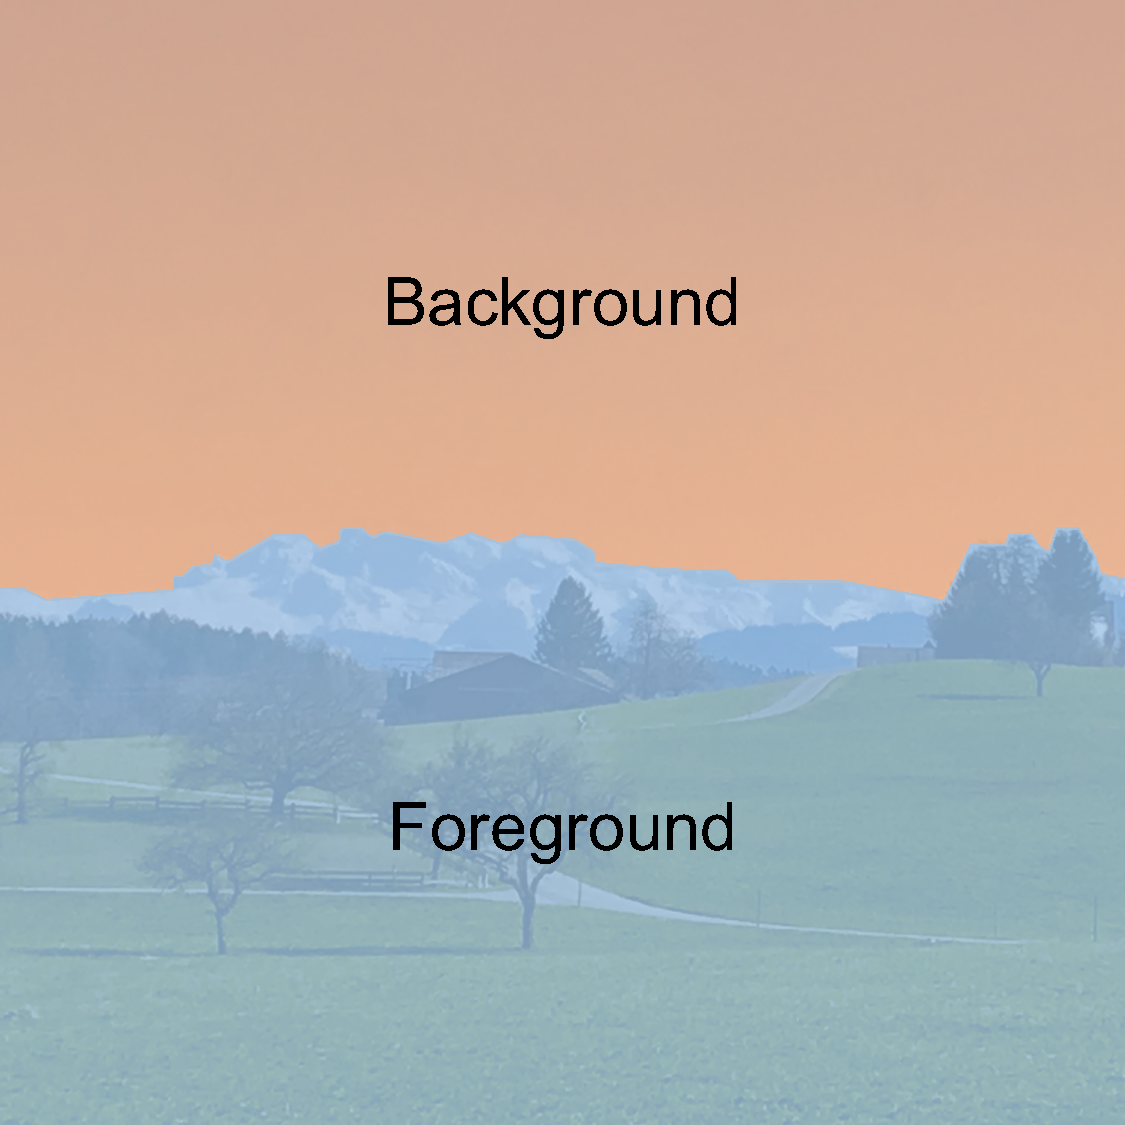
\includegraphics[width=\figfig\textwidth]{1-01-1.pdf}
	}
    \caption[Example of binary image segmentation]{Example of image binary segmentation. The original image (a) is taken from Uetzgi Takeoff.}
	\label{fig:eg01imgseg}
\end{figure}

\subsection{Geometrical Shape}\label{geosha}

我们想要脱离每像素标签,并直接通过向量表示学习多边形。当我们偏离标注像素的标准范例并旨在直接利用和学习建筑物的几何形状时
-多边形表示包括比像素方式标签少得多的冗余
-在存储上有优势
-可以矢量表示,即在不同层面都可以用	,建筑物等对象可以更自然地建模
-学习到的多边形可以直接标注在电子地图中,而像素的不行
因此多边形表示是感兴趣对象的更紧凑和有用的表示。因此我们希望能够从航拍图像中获取多边形
最近,深度学习方法在诸如图像分割和对象检测等许多计算机视觉任务中展现出了显着的成就。而相关方法已经被应用于航拍图像中[10,11,12,13,14],但是,这些传统的CNN架构仍然局限于常规的网格结构图。这些网络的僵化使得很难开发关于图像内容的高级先验。他们输出的结果仍然是pixel wise的。那么,如何快速地从航拍图像中检测出矢量图变成了一大问题。
总之,这个项目的目的是为图形和任意结构的几何形状开发新颖的深度学习方法,我们试图将对象拓扑和形状引入深度学习技术。我们想要脱离标注像素的标准范例,而是直接利用并学习对象的几何图形。

\section{Problem Definition}\label{prodef}


(给图)给定一张航拍图,为航拍图中的每一个房屋,寻找它的多边形shape。输入是什么……输出是什么……

Instance segmentation is challenging because it requires the correct detection of all objects in an image while also precisely segmenting each instance. It therefore combines elements from the classical computer vision tasks of ob- ject detection, where the goal is to classify individual ob- jects and localize each using a bounding box, and semantic segmentation, where the goal is to classify each pixel into a fixed set of categories without differentiating object in- stances.
\section{Focus of This Work}\label{fcswrk}

为了解决这个问题,本文提出的模型叫region-based PolygonRNN。它是结合了Mask R-CNN中的FPN部分和PolygonRNN的产物。其中,FPN用于进行定位,即检测图像中的RoI,PolygonRNN部分用于find geometric shape。

\section{Thesis Organization}\label{thsorg}

本论文组织如下。首先,我们回顾相关工作2 并着眼于像素级别的方法和bbox回归的方法(previous thesis)。并且看一下最近的新模型——mask r-cnn和单个polygon的
在第3章中,两个新模型的具体架构将会被讨论。成功的对象检测算法Faster R-CNN将在第4章中解释,因为它作为我们在第5章中描述的第一种建筑物分割方法的基础。我们的第二种建筑物分割方法基于建筑物角点提取,其后是连体网络来检测属于同一建筑物的匹配角落。这个方法的描述可以在第6章中找到。我们在第7章中对这两种方法进行了评估。在上一章中对结论进行了描述并对未来的工作进行了讨论。

Following common terminology, we use object detection to denote detection via bounding boxes, not masks, and semantic segmentation to denote per-pixel classification without differentiating instances. Yet we note that instance segmentation is both semantic and a form of detection.
